\section{Préliminaires}
  \subsection{Cadre du Plan d’Assurance Qualité Projet (ou PAQP}
  Le PAQP est mis en place dans le cadre de la réponse à l'appel d'offre "Système de monitoring à distance de sites isolés" par l'hexanôme H4212 (Maitrise d'oeuvre ou MOE) lancé par le COPEVUE.

\par Toute la documentation fournie par la MOE durant le projet est concernée par ce PAQP ainsi que tout sous-projet.

  \subsection{Objectif du Plan d’Assurance Qualité Projet}
    \subparagraph{La mise en place d'un système de qualité} tout au long de la conduite du projet. Ce PAQP doit être mis en oeuvre par la MOE afin de satisfaire la maitrise d'ouvrage.
    \subparagraph{L'assurance de la cohérence et de l'homogénéité des documents} et livrables produits. le PAQP est mis en place pour assurer la qualité du produit fini.

  \subsection{Responsabilités associées au Plan d’Assurance Qualité Projet}                        
L'ensemble des membres de la MOE est concerné par le PAQP. Pour la bonne conduite du projet, il est obligatoire que le PAQP soit connu de tous, et qu'il soit appliqué. Cependant, chaque personne a un rôle différent vis-à-vis du PAQP :

\paragraph{Groupe d'Etude Informatique (GEI)\\}	 
                \begin{itemize}
                \item Appliquer le PAQP
                \item Corriger les documents non-conformes pour être en conformité avec le PAQP
                \end{itemize}

\paragraph{Responsable Qualité (RQ)\\}
                \begin{itemize}
                \item Rédiger et améliorer le PAQP
                \item Garantir l'application du PAQP
                \end{itemize}	
                
\paragraph{Chef de Projet(CdP)\\} 
                \begin{itemize}
                \item Appliquer le PAQP
                \item Valider le PAQP
                \item Faire respecter le PAQP
                \end{itemize}
    
  \subsection{Procédures d’évolution du PAQP}

Il appartient à chacun de faire évoluer le PAQP. Par définition, le PAQP est voué à évoluer pour s'améliorer afin d'atteindre le "Zero Defaut".
\par Le PAQP peut-être amené à évoluer pour plusieurs raisons : 
\begin{itemize}
\item détection d'un défaut ou d'une imprécision dans le PAQP 
\item découverte d'une "Best-Practice" qui peut être source d'inspiration pour le présent PAQP 
\item mise en place d'une nouvelle règle, d'un nouvel outil,...\\
\end{itemize}

Toute évolution doit être soumise au RQ, qui la prendra en considération, et qui devra être validée par le CdP. 
Lorsqu'une procédure d'évolution du PAQP aboutie, tous les membres du projet sont avertis et informés.

  \subsection{Procédure à suivre en cas de non-application du PAQP}

Première régle importante : lorsqu'un document, résultat ou livrable produit par l'équipe du projet ne respecte pas le PAQP, il ne pourra pas être validé.

L'auteur de la non-conformité doit être averti par le RQ et/ou le CdP, et il lui sera fourni les éléments et informations nécessaires à la correction. Ce dernier devra alors prendre en compte ces informations, et procéder aux modifications nécessaires, pour que le document produit puisse être définitivement validé.

  \subsection{Procédure de dérogation du PAQP}
Une certaine flexibilité dans l'application du PAQP est envisageable. Il ne s'agit d'être rigoriste.

De ce fait, si un membre de l'équipe du projet, pour un document, résultat ou livrable en cours de production, juge opportuniste pour des raisons données de ne pas appliquer des règles du PAQP, il peut en faire part au RQ, avec des justification.

En fonction des justifications, le RQ prend la décision d'accorder ou pas la dérogation. En cas de dérogation, il en averti le CdP. Si le membre du projet se voit refuser sa dérogation, il peut, s'il le juge opportun, solliciter le CdP, qui tranchera.
\section{Documents de Référence et applicables}
  \subsection{Documents de référence}
  \begin{center} \begin{Large}TODO\end{Large}  \end{center}
  \subsection{Documents Applicables}
  \begin{center} \begin{Large}TODO\end{Large}  \end{center}

\section{Terminologies et abréviations}
\noindent CdC : Cahier des Charges \\
CdP : Chef de Projet\\       
GEI : Groupe d'Etude Informatique\\ 
MOA : Maitrise d'ouvrage\\      
MOE : Maitrise d'oeuvre\\
RQ : Responsable Qualité\\    
PAQP : Plan d’Assurance Qualité Projet
                                                                     
\section{Organisation humaine du comité de pilotage du projet} 
  \subsection{Rôle des différents intervenants ( Intervenants pour la maîtrise d’ouvrage, intervenants pour la maîtrise d’œuvre)}
\paragraph{COPEVUE (client)}il s'agit de la socièté à l'origine de l'appel d'offre "Système de monitoring à distances de sites isolés".
\paragraph{MOA}La MOA dépend de la COPEVUE. Elle est responsable du CdC, et veille à son respect par la MOE. Elle valide le travail de la MOE.
\paragraph{MOE}Il s'agit de l'hexanôme H4212. Il est chargé de répondre à l'appel d'offre de COPEVUE. La MOE est responsable du déroulement du projet et de la solution proposée, tout en tenant compte des contraintes du CdC et des délais fixés par la MOA. Il existe au sein de la MOE plusieurs acteurs :

\subparagraph{CdP}Dirige le projet, et l'équipe de la MOE par la mise en place d'outils de gestion de projet. Il s'occupe d'affecter des ressources à des tâches. Il est le garant du bon déroulement du projet. Il est aussi le lien entre la MOA et la MOE.
\subparagraph{RQ}s'occupe de la démarche qualité au sein du projet. Il doit rédiger et faire respecter différents documents(PAQP, Gestion de de la Documentation,...). Il est le garant du Système Qualité.
\subparagraph{GEI}Effectue des études et produit de la documentation en fonction des tâches affectées par le CdP. La documentation produite doit respecter les différentes règles du Système Qualité.

  \subsection{Relations entre les intervenants}
  \begin{center} \begin{Large}TODO Organigramme\end{Large}  \end{center}
  \subsection{Planning des réunions et règles}
  C'est la MOA qui doit régir les différentes deadlines. Pour cela, elle doit communiquer l'ensemble des dates importantes au bon déroulement du projet à la MOE. le planning global du déroulement du projet doit être connu dès le début, pour que la MOE s'engage à respecter à la lettre ce planning. Ces dates correspondent soit aux dates de revues intermédiaires soit aux dates de remises des différents livrables.
Les différentes revues intermédiaires permettront de valider les différents résultats produits par la MOE, d'apporter des critiques, de faire des demandes de modification et éventuellement d'affiner et/ou corriger le CdC de la MOA en fonction des problèmes/questions soulevées.

\section{Qualité au niveau du Processus}
  \subsection{Présentation de la démarche de développement au niveau Système}
  
    \subsubsection{Généralités}
     Le développement de ce système se basera sur IEEE 1220, qui produit des livrables à la fin de chacune des phases du cycle et divise le système en sous-projets au moment de l'étude détaillée.
     Notre projet se prête bien à la division en sous-systèmes (on pense par exemple au sous-système "Système Embarqué sur les sites génériques" ou encore "Gestion de l'énergie").  \\
     
     \begin{center}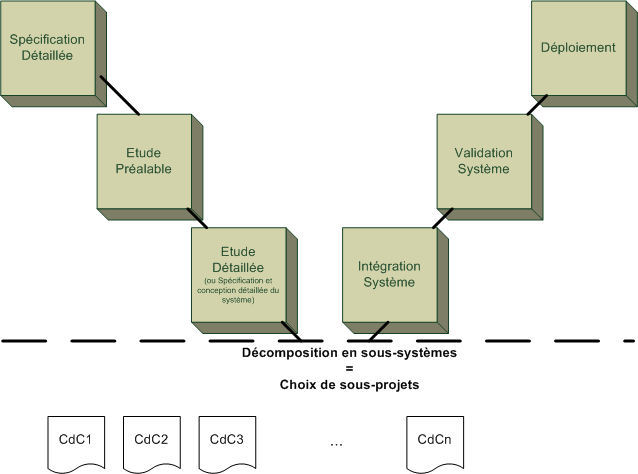
\includegraphics [width=0.7\textwidth]{IEEE1020.png}\end{center}


\subsubsection{Spécification détaillée}
Cette phase consiste à étudier de manière précise et détaillée les besoins du client. C'est faire une étude de l'existant et une spécification des objectifs du système.

1.8.2.4   Codage et analyse statique
Lors de cette phase, développement des différents sous-composants listés lors des phases précédentes.  

    \subsubsection{Phase d’Etude Préalable}
  Durant cette phase, il peut être nécessaire de commencer par l'ébauche de plusieurs variantes de solutions et choisir celle qui répond le mieux aux besoins spécifiés lors de la phase précédente tout en tenant compte des contraintes (coûts, etc.) La solution retenue sera ensuite figée, d'où l'importance de cette phase. En parallèle, lors de cette phase, un plan d'intégration et un plan de tests sont élaborés.
    
    \subsubsection{Phase d’Etude Détaillée}
    Cette phase sert à détailler ce qui a été donné dans la phase précédente, en divisant le système en sous-projets. Cette décomposition est faite jusqu'à obtenir des entités faciles à tester et à implémenter.

    Les sous-projets sont ensuites régies par leur propre méthode de développement (l'un peut suivre la méthode AGILE l'autre maquettage-prototypage, selon ce qui parait le plus adéquat). Les seuls obligations sont que chaque sous-systèmes doit respecter le Plan d'Assurance Qualité du Projet.
    Chaque sous-projet, de par leur méthode de développement, est testé (indépendamment des autres).
    
    \subsubsection{Phase d’Intégration Système }
    L'ensemble des sous-systèmes sont intégrés et le système est alors testé.
    \subsubsection{Phase de Validation Système}
    Vérification et validation de la conformité du système par rapport au CdC par le client.
    \subsubsection{Phase de Déploiement}
    Réception du système par le client et déploiement du nouveau système sur le site.





\subsection{Règles de Qualité pour l’ingénierie concurrente}
\begin{center} \begin{Large}KESAKO?\end{Large}  \end{center}
\subsubsection{Règles sur la rédaction d’un Cahier des Charges d’un sous-projet}
\subsubsection{Règles sur la définition précise des résultats attendus pour chaque sous-projets}
\subsubsection{Règles sur le suivi qualité des sous-projets}
\subsubsection{Règles sur la définition de critères d’acceptation des sous-projets avant intégration}
\subsection{Présentation des démarche de développement au niveau sous-projets (niv. réalisation)}
\subsubsection{Liste des processus de développement susceptibles d’être retenus pour le développement des sous-projets}
\subsubsection{Description du cycle de développement n°1}
\begin{itemize}
  \item Liste des étapes
  \item Pour étape n°J
  \item Documents en entrée
  \item Documents en sortie
  \item Conditions de validation de l’étape
  \item Suivi de projet
\end{itemize}
















 
\section{Documentation (Règles communes au projet)}
\begin{center} \begin{Large}Ce chapitre reprend en partie le document Gestion de la Documentation. Il ne sera donc pas traité\end{Large}  \end{center}
\subsection{Structuration de la documentation}
\subsection{Liste des documents de gestion de projet}
\subsection{Liste des documents relatifs à la qualité}
\subsection{Liste des documents techniques et de réalisation}
\subsection{Manuels d’utilisation et de mise en œuvre}

\section{Gestion de configuration (Règles communes au projet)}
  \subsection{Convention d’utilisation}
   La gestion de configuration s'applique à l'ensemble du projet. Elle permet d'assurer la cohérence, le partage et le stockage des différents documents produits.
Durant notre projet nous utiliserons l'outil Git sur la plateforme Github (http://www.github.com/).

  \subsection{Responsabilités}
    Le RQ sera responsable de la mis en place de l'outil de gestion de configuration, de ses réglages et de sa maintenance.
    Les différents membres du projet devront maîtriser l'outil. Pour cela, se référer à la documentation officielle de l'outil.
  \subsection{Gestion des ressources partagées}
  L'ensemble des ressources qui seront présentes sur l'outil Git seront partagées.
  
\section{Gestions des modifications  (Règles communes au projet)}
  \subsection{Origines des modifications}
  \begin{center} \begin{Large}TODO\end{Large}  \end{center}
  \subsection{Procédures et organisation des modifications}
  \begin{center} \begin{Large}TODO\end{Large}  \end{center}


\section{Contrôle des Fournisseurs}
  \subsection{Exigences vis-à-vis des sous-traitants}
    \begin{center} \begin{Large}TODO\end{Large}  \end{center}
  \subsection{Exigences vis-à-vis des co-traitants}
    \begin{center} \begin{Large}TODO\end{Large}  \end{center}
  \subsection{Logiciels achetés, loués ou imposés}
    \begin{center} \begin{Large}TODO\end{Large}  \end{center}

\section{Reproduction, Protection, Livraison (au niveau projet)}
  \subsection{Précautions à prendre lors de la reproduction}
      \begin{center} \begin{Large}TODO\end{Large}  \end{center}
  \subsection{Précautions prises pour assurer le stockage des logiciels}
    \subsubsection{Protection des données contre les incidents}
        \begin{center} \begin{Large}TODO\end{Large}  \end{center}
    \subsubsection{Protection des données contre les agressions extérieures}
        \begin{center} \begin{Large}TODO\end{Large}  \end{center}
    \subsubsection{Autres précautions}
        \begin{center} \begin{Large}TODO\end{Large}  \end{center}
  \subsection{Modalités de livraison}
    \subsubsection{Délais}
    \begin{center} \begin{Large}TODO\end{Large}  \end{center}
    \subsubsection{Installation}
    \begin{center} \begin{Large}TODO\end{Large}  \end{center}
    \subsubsection{Formation}
    \begin{center} \begin{Large}TODO\end{Large}  \end{center}
    \subsubsection{Migration de l’ancien vers le nouveau système}
    \begin{center} \begin{Large}TODO\end{Large}  \end{center}

\section{Suivi de l’application du Plan Qualité}
    \subsection{Principes}
    L'application du plan qualité est primordiale si l'on souhaite effectuer un travail de qualité et produire des livrables respectant une certaine homogénéité et cohérence.
    L'assurance qualité concerne toutes les procédures qualité établies par le RQ.
    \subsection{Interventions du Responsable Qualité (Niv. Projet) sur la démarche de Développement}
    Lors des différentes phases de développement du projet, le RQ a pour principales responsabilités: - Le support qualité auprès de l'équipe projet - la validation de la forme des documents produits et livrés selon les règles énoncées dans la Gestion de la Documentation. - la vérification du suivi et de l'application du PAQP par l'équipe projet - la création, le maintien et l'évolution du Système Qualité.
    
    \begin{center} \begin{Large}TODO\end{Large}  \end{center}
  \subsection{Modalités de réception des résultats des sous-projets avant intégration	( description par sous-projets)}
      \begin{center} \begin{Large}TODO\end{Large}  \end{center}
\section{Conclusion}
Ce PAQP est un document et un outil qui permet de garantir une solution finale de qualité, à condition qu'il soit bien appliqué.
Il permet également d'assurer la prise en compte des attentes du client.
La Qualité a pour vocation d'être toujours améliorée, le présent document doit être sujet à une modification permanente.